% TODO: would benefit from more of a third person writing prose.
% i.e: we are currently talking in terms of "we did X and found Y" rather than
% "because of hyp Z, we tried X and found Y, shown in fig A"
% feels a bit "aimless" of a scientific approach.

\subsection{Unconditional Image Generation}
\label{subsec:evaluationUnconditional}

\begin{figure}
    \centering
    \begin{subfigure}[b]{0.33\textwidth}
        \centering
        \resizebox{\textwidth}{!}{
            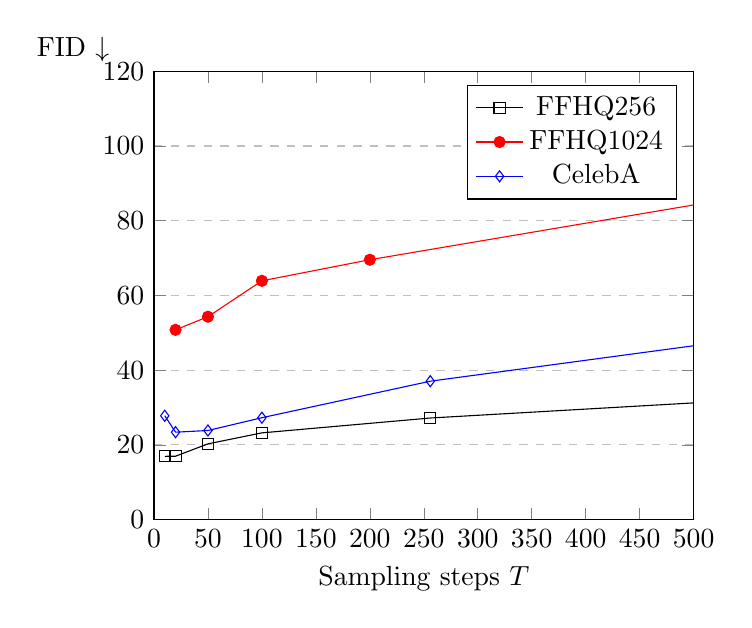
\begin{tikzpicture}
\begin{axis}[
y label style={at={(axis description cs:-0.15,1.0)},rotate=-90,anchor=south},
title={},
xlabel={Sampling steps $T$},
ylabel={FID $\downarrow$},
xmin=0, xmax=500,
ymin=0, ymax=120,
xtick={0,50,100,150,200,250,300,350,400,450,500},
ytick={0,20,40,60,80,100,120},
legend pos=north east,
ymajorgrids=true,
grid style=dashed,
]\addplot[color=black, mark=square]
coordinates {(10.0, 16.933240853331633)(20.0, 16.968015496794585)(50.0, 20.269439432847413)(100.0, 23.214299375538577)(256.0, 27.189009006094718)(512.0, 31.435942790814245)};
\addlegendentry{FFHQ256}
\addplot[color=red, mark=*]
coordinates {(20.0, 50.79169256114352)(50.0, 54.30311107720983)(100.0, 63.90726480083863)(200.0, 69.5533429056805)(512.0, 84.80617604620527)(1024.0, 100.93734948403663)};
\addlegendentry{FFHQ1024}
\addplot[color=blue, mark=diamond]
coordinates {(10.0, 27.79389706651663)(20.0, 23.397719254573232)(50.0, 23.845846223411986)(100.0, 27.26720576724899)(256.0, 37.0436486740923)(512.0, 46.99500404006332)};
\addlegendentry{CelebA}
\end{axis}
\end{tikzpicture}

        }
        \caption{Steps vs. FID}
    \end{subfigure}
    \hfill
    \begin{subfigure}[b]{0.33\textwidth}
        \centering
        \resizebox{\textwidth}{!}{
            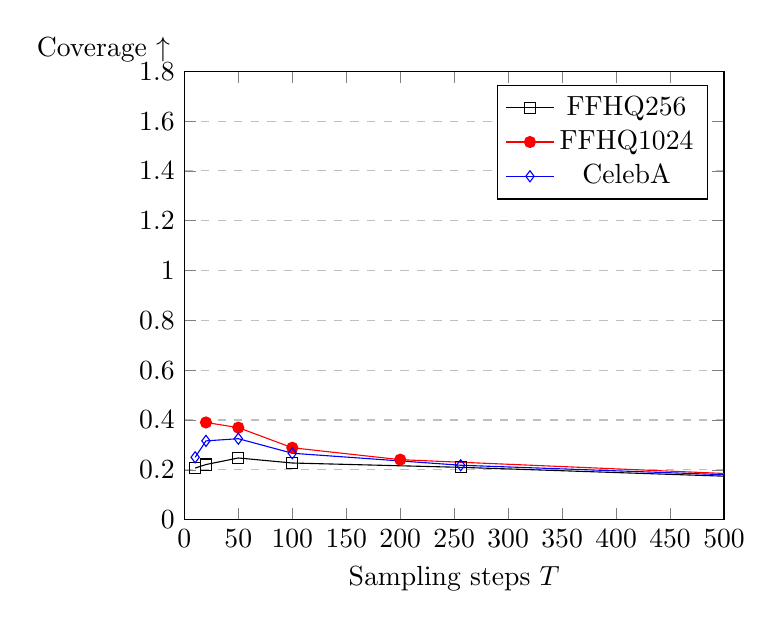
\begin{tikzpicture}
\begin{axis}[
y label style={at={(axis description cs:-0.15,1.0)},rotate=-90,anchor=south},
title={},
xlabel={Sampling steps $T$},
ylabel={Coverage $\uparrow$},
xmin=0, xmax=500,
ymin=0.0, ymax=1.8,
xtick={0,50,100,150,200,250,300,350,400,450,500},
ytick={0.0,0.2,0.4,0.6000000000000001,0.8,1.0,1.2000000000000002,1.4000000000000001,1.6,1.8},
legend pos=north east,
ymajorgrids=true,
grid style=dashed,
]\addplot[color=black, mark=square]
coordinates {(10.0, 0.207)(20.0, 0.221)(50.0, 0.2474)(100.0, 0.2272)(256.0, 0.2098)(512.0, 0.1726)};
\addlegendentry{FFHQ256}
\addplot[color=red, mark=*]
coordinates {(20.0, 0.39)(50.0, 0.3692)(100.0, 0.2884)(200.0, 0.2406)(512.0, 0.183)(1024.0, 0.1448)};
\addlegendentry{FFHQ1024}
\addplot[color=blue, mark=diamond]
coordinates {(10.0, 0.2502)(20.0, 0.316)(50.0, 0.3248)(100.0, 0.2664)(256.0, 0.2182)(512.0, 0.1784)};
\addlegendentry{CelebA}
\end{axis}
\end{tikzpicture}

        }
        \caption{Steps vs. Coverage}
    \end{subfigure}
    \hfill
    \begin{subfigure}[b]{0.33\textwidth}
        \centering
        \resizebox{\textwidth}{!}{
            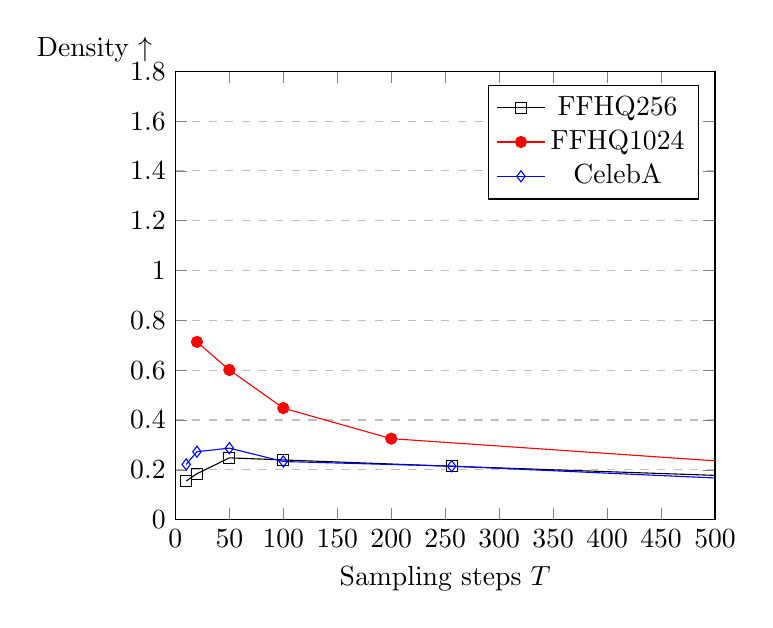
\begin{tikzpicture}
\begin{axis}[
y label style={at={(axis description cs:-0.15,1.0)},rotate=-90,anchor=south},
title={},
xlabel={Sampling steps $T$},
ylabel={Density $\uparrow$},
xmin=0, xmax=500,
ymin=0.0, ymax=1.8,
xtick={0,50,100,150,200,250,300,350,400,450,500},
ytick={0.0,0.2,0.4,0.6000000000000001,0.8,1.0,1.2000000000000002,1.4000000000000001,1.6,1.8},
legend pos=north east,
ymajorgrids=true,
grid style=dashed,
]\addplot[color=black, mark=square]
coordinates {(10.0, 0.155)(20.0, 0.18413333333333332)(50.0, 0.24793333333333334)(100.0, 0.23946666666666666)(256.0, 0.21406666666666666)(512.0, 0.17573333333333332)};
\addlegendentry{FFHQ256}
\addplot[color=red, mark=*]
coordinates {(20.0, 0.7133333333333334)(50.0, 0.6008666666666667)(100.0, 0.44753333333333334)(200.0, 0.3249333333333333)(512.0, 0.2324)(1024.0, 0.16773333333333332)};
\addlegendentry{FFHQ1024}
\addplot[color=blue, mark=diamond]
coordinates {(10.0, 0.2215333333333333)(20.0, 0.2724)(50.0, 0.2869333333333333)(100.0, 0.2332)(256.0, 0.21446666666666664)(512.0, 0.16473333333333331)};
\addlegendentry{CelebA}
\end{axis}
\end{tikzpicture}

        }
        \caption{Steps vs. Density}
    \end{subfigure}
    \caption{
        Plots showing sample quality in terms of different metrics as
        number of sampling steps $\markovSteps$ increases. Counter-intuitively, the
        sample quality decreases with number of sampling steps, seen on
        all metrics and datasets.
    }
    \label{fig:step}
\end{figure}

\begin{figure}
    \begin{subfigure}[b]{0.33\textwidth}
        \centering
        \resizebox{\textwidth}{!}{
            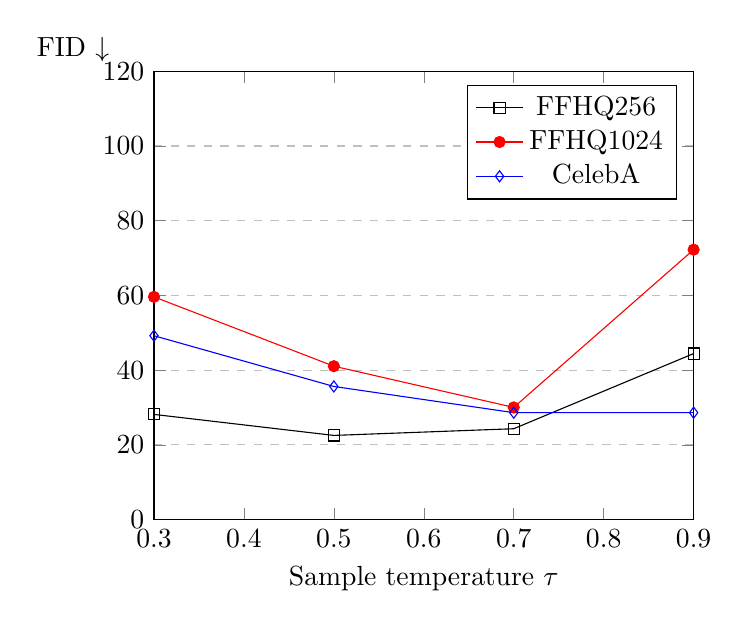
\begin{tikzpicture}
\begin{axis}[
y label style={at={(axis description cs:-0.15,1.0)},rotate=-90,anchor=south},
title={},
xlabel={Sample temperature $\tau$},
ylabel={FID $\downarrow$},
xmin=0.3, xmax=0.9000000000000001,
ymin=0, ymax=120,
xtick={0.3,0.4,0.5,0.6000000000000001,0.7000000000000002,0.8000000000000003,0.9000000000000001},
ytick={0,20,40,60,80,100,120},
legend pos=north east,
ymajorgrids=true,
grid style=dashed,
]\addplot[color=black, mark=square]
coordinates {(1.0, 83.59790014438649)(0.9, 44.43439367176743)(0.7, 24.322136621661407)(0.5, 22.530204016446124)(0.3, 28.155348332963445)};
\addlegendentry{FFHQ256}
\addplot[color=red, mark=*]
coordinates {(1.0, 281.35575866892975)(0.9, 72.24972119845785)(0.7, 30.030630965588852)(0.5, 41.06155796980428)(0.3, 59.61624309496067)};
\addlegendentry{FFHQ1024}
\addplot[color=blue, mark=diamond]
coordinates {(1.0, 75.80203954506536)(0.9, 28.617311837121477)(0.7, 28.621503391331398)(0.5, 35.63571015802388)(0.3, 49.21726306807049)};
\addlegendentry{CelebA}
\end{axis}
\end{tikzpicture}

        }
        \caption{Temperature $\temperature$ vs. FID}
    \end{subfigure}
    \hfill
    \begin{subfigure}[b]{0.33\textwidth}
        \centering
        \resizebox{\textwidth}{!}{
            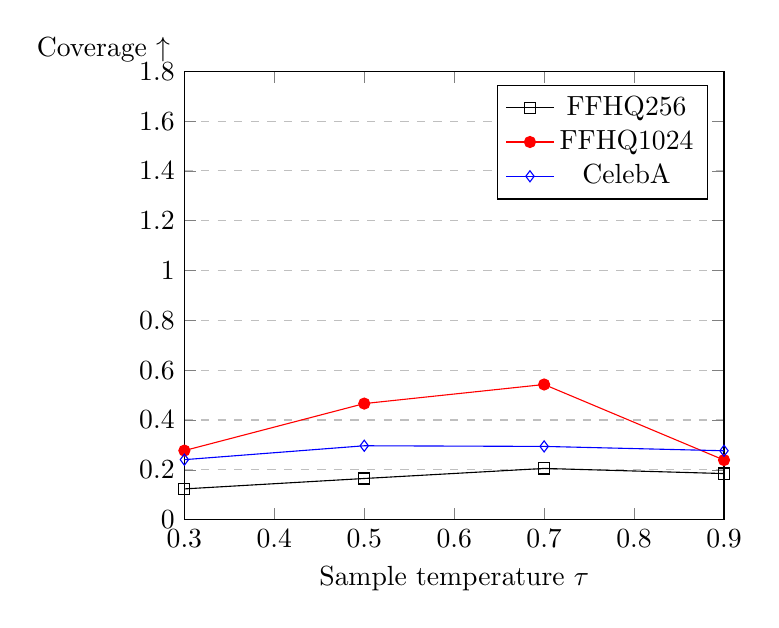
\begin{tikzpicture}
\begin{axis}[
y label style={at={(axis description cs:-0.15,1.0)},rotate=-90,anchor=south},
title={},
xlabel={Sample temperature $\tau$},
ylabel={Coverage $\uparrow$},
xmin=0.3, xmax=0.9000000000000001,
ymin=0.0, ymax=1.8,
xtick={0.3,0.4,0.5,0.6000000000000001,0.7000000000000002,0.8000000000000003,0.9000000000000001},
ytick={0.0,0.2,0.4,0.6000000000000001,0.8,1.0,1.2000000000000002,1.4000000000000001,1.6,1.8},
legend pos=north east,
ymajorgrids=true,
grid style=dashed,
]\addplot[color=black, mark=square]
coordinates {(1.0, 0.0662)(0.9, 0.1848)(0.7, 0.2054)(0.5, 0.165)(0.3, 0.1232)};
\addlegendentry{FFHQ256}
\addplot[color=red, mark=*]
coordinates {(1.0, 0.0004)(0.9, 0.239)(0.7, 0.5424)(0.5, 0.4658)(0.3, 0.277)};
\addlegendentry{FFHQ1024}
\addplot[color=blue, mark=diamond]
coordinates {(1.0, 0.124)(0.9, 0.2764)(0.7, 0.2938)(0.5, 0.2964)(0.3, 0.2406)};
\addlegendentry{CelebA}
\end{axis}
\end{tikzpicture}

        }
        \caption{Temperature $\temperature$ vs. Coverage}
    \end{subfigure}
    \hfill
    \begin{subfigure}[b]{0.33\textwidth}
        \centering
        \resizebox{\textwidth}{!}{
            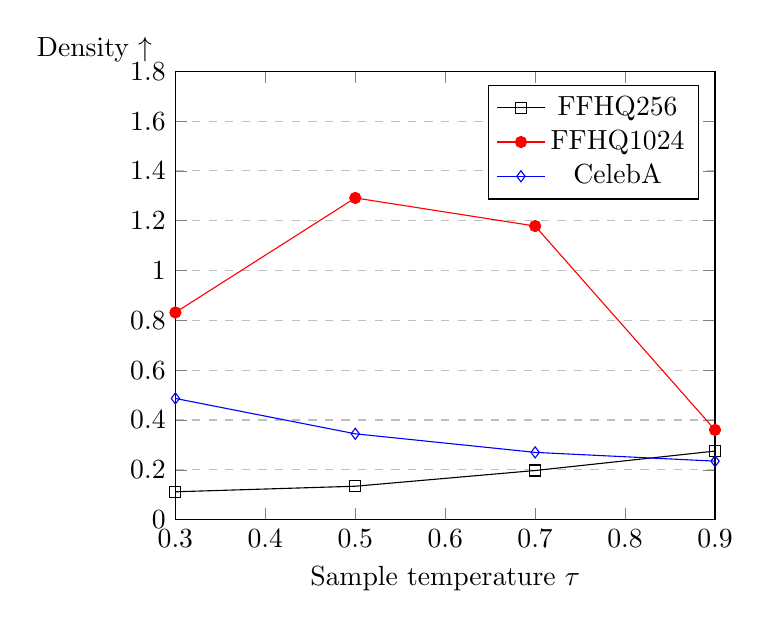
\begin{tikzpicture}
\begin{axis}[
y label style={at={(axis description cs:-0.15,1.0)},rotate=-90,anchor=south},
title={},
xlabel={Sample temperature $\tau$},
ylabel={Density $\uparrow$},
xmin=0.3, xmax=0.9000000000000001,
ymin=0.0, ymax=1.8,
xtick={0.3,0.4,0.5,0.6000000000000001,0.7000000000000002,0.8000000000000003,0.9000000000000001},
ytick={0.0,0.2,0.4,0.6000000000000001,0.8,1.0,1.2000000000000002,1.4000000000000001,1.6,1.8},
legend pos=north east,
ymajorgrids=true,
grid style=dashed,
]\addplot[color=black, mark=square]
coordinates {(1.0, 0.07566666666666666)(0.9, 0.2750666666666667)(0.7, 0.19706666666666664)(0.5, 0.13393333333333332)(0.3, 0.11159999999999999)};
\addlegendentry{FFHQ256}
\addplot[color=red, mark=*]
coordinates {(1.0, 0.00019999999999999998)(0.9, 0.3599333333333333)(0.7, 1.1785333333333332)(0.5, 1.2913999999999999)(0.3, 0.8315333333333333)};
\addlegendentry{FFHQ1024}
\addplot[color=blue, mark=diamond]
coordinates {(1.0, 0.12519999999999998)(0.9, 0.23466666666666663)(0.7, 0.26986666666666664)(0.5, 0.3444666666666667)(0.3, 0.4864)};
\addlegendentry{CelebA}
\end{axis}
\end{tikzpicture}

        }
        \caption{Temperature $\temperature$ vs. Density}
    \end{subfigure}
    \caption{
        Plots showing sample quality in terms of different metrics as sample
        temperature $\temperature$ is changed. Given the other parameters, a good choice
        of $\temperature$ falls in the range $0.5-0.7$. However, this range may
        differ depending on the other choice of parameters.
    }
    \label{fig:temp}
\end{figure}

\begin{figure}
    \begin{subfigure}[b]{0.33\textwidth}
        \centering
        \resizebox{\textwidth}{!}{
            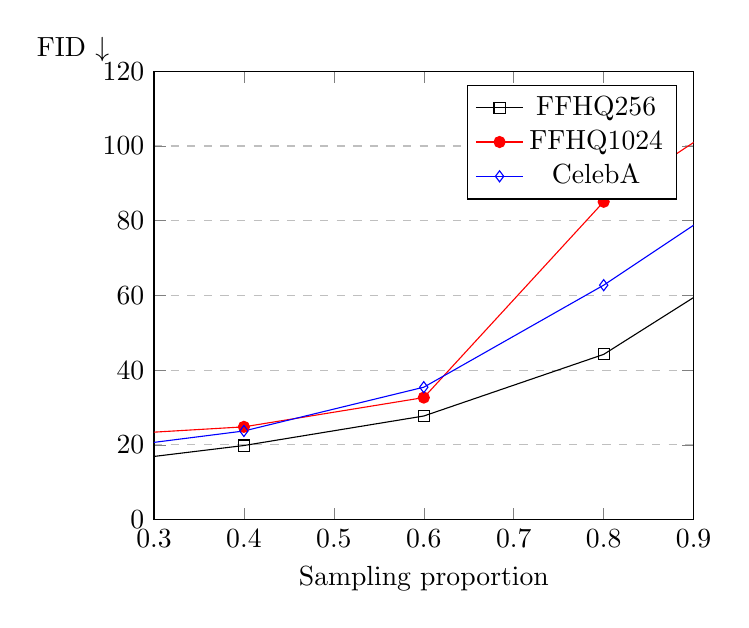
\begin{tikzpicture}
\begin{axis}[
y label style={at={(axis description cs:-0.15,1.0)},rotate=-90,anchor=south},
title={},
xlabel={Sampling proportion},
ylabel={FID $\downarrow$},
xmin=0.3, xmax=0.9000000000000001,
ymin=0, ymax=120,
xtick={0.3,0.4,0.5,0.6000000000000001,0.7000000000000002,0.8000000000000003,0.9000000000000001},
ytick={0,20,40,60,80,100,120},
legend pos=north east,
ymajorgrids=true,
grid style=dashed,
]\addplot[color=black, mark=square]
coordinates {(1.0, 74.66283778948849)(0.8, 44.21927055440783)(0.6, 27.725188336835213)(0.4, 19.825740890874904)(0.2, 13.976620506685805)};
\addlegendentry{FFHQ256}
\addplot[color=red, mark=*]
coordinates {(1.0, 116.81614755529716)(0.8, 85.06652266724691)(0.6, 32.65933412137353)(0.4, 24.82419203797879)(0.2, 21.979835694569083)};
\addlegendentry{FFHQ1024}
\addplot[color=blue, mark=diamond]
coordinates {(1.0, 94.83723271911529)(0.8, 62.7489179950907)(0.6, 35.43514345702618)(0.4, 23.718088259439654)(0.2, 17.614758693266793)};
\addlegendentry{CelebA}
\end{axis}
\end{tikzpicture}

        }
        \caption{Sample proportion vs. FID}
    \end{subfigure}
    \hfill
    \begin{subfigure}[b]{0.33\textwidth}
        \centering
        \resizebox{\textwidth}{!}{
            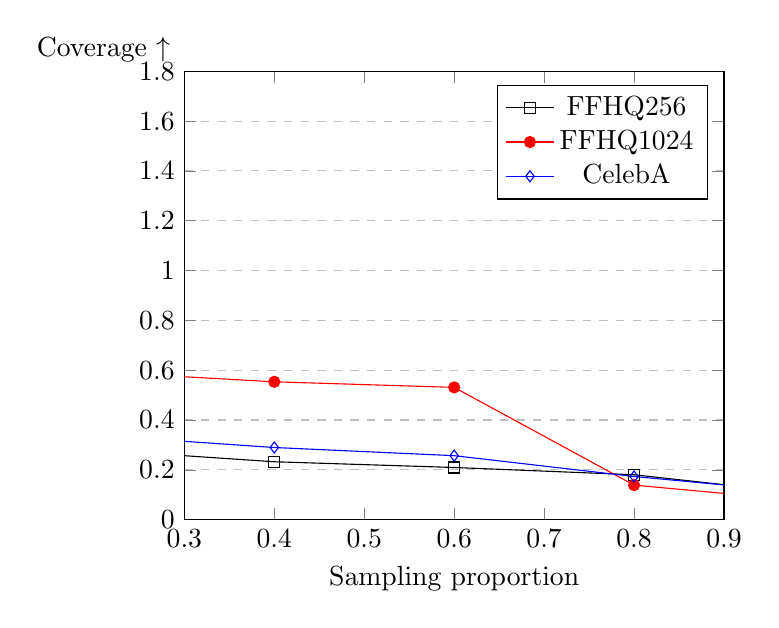
\begin{tikzpicture}
\begin{axis}[
y label style={at={(axis description cs:-0.15,1.0)},rotate=-90,anchor=south},
title={},
xlabel={Sampling proportion},
ylabel={Coverage $\uparrow$},
xmin=0.3, xmax=0.9000000000000001,
ymin=0.0, ymax=1.8,
xtick={0.3,0.4,0.5,0.6000000000000001,0.7000000000000002,0.8000000000000003,0.9000000000000001},
ytick={0.0,0.2,0.4,0.6000000000000001,0.8,1.0,1.2000000000000002,1.4000000000000001,1.6,1.8},
legend pos=north east,
ymajorgrids=true,
grid style=dashed,
]\addplot[color=black, mark=square]
coordinates {(1.0, 0.1002)(0.8, 0.18)(0.6, 0.2092)(0.4, 0.2322)(0.2, 0.2808)};
\addlegendentry{FFHQ256}
\addplot[color=red, mark=*]
coordinates {(1.0, 0.0718)(0.8, 0.1384)(0.6, 0.5308)(0.4, 0.5532)(0.2, 0.5936)};
\addlegendentry{FFHQ1024}
\addplot[color=blue, mark=diamond]
coordinates {(1.0, 0.1054)(0.8, 0.173)(0.6, 0.2566)(0.4, 0.2894)(0.2, 0.3392)};
\addlegendentry{CelebA}
\end{axis}
\end{tikzpicture}

        }
        \caption{Sample proportion vs. Coverage}
    \end{subfigure}
    \hfill
    \begin{subfigure}[b]{0.33\textwidth}
        \centering
        \resizebox{\textwidth}{!}{
            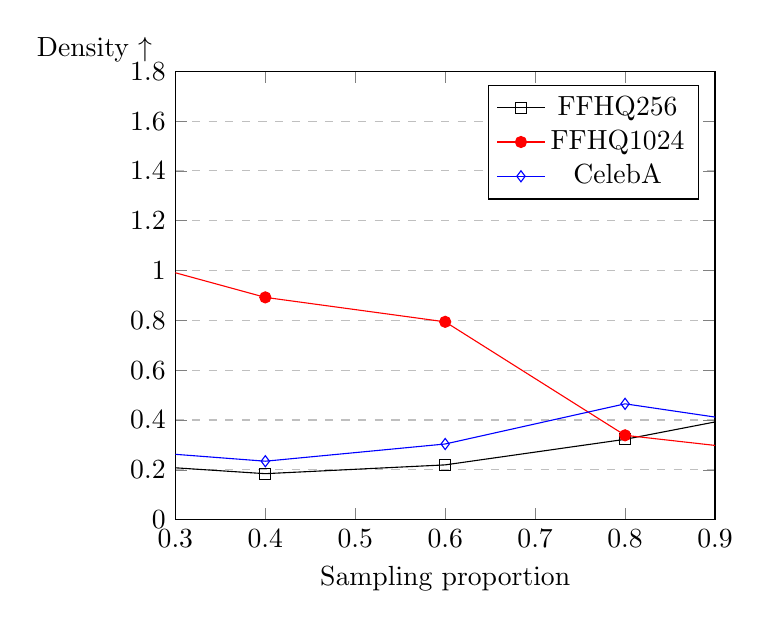
\begin{tikzpicture}
\begin{axis}[
y label style={at={(axis description cs:-0.15,1.0)},rotate=-90,anchor=south},
title={},
xlabel={Sampling proportion},
ylabel={Density $\uparrow$},
xmin=0.3, xmax=0.9000000000000001,
ymin=0.0, ymax=1.8,
xtick={0.3,0.4,0.5,0.6000000000000001,0.7000000000000002,0.8000000000000003,0.9000000000000001},
ytick={0.0,0.2,0.4,0.6000000000000001,0.8,1.0,1.2000000000000002,1.4000000000000001,1.6,1.8},
legend pos=north east,
ymajorgrids=true,
grid style=dashed,
]\addplot[color=black, mark=square]
coordinates {(1.0, 0.46173333333333333)(0.8, 0.32226666666666665)(0.6, 0.21966666666666668)(0.4, 0.18433333333333335)(0.2, 0.23146666666666665)};
\addlegendentry{FFHQ256}
\addplot[color=red, mark=*]
coordinates {(1.0, 0.25726666666666664)(0.8, 0.33840000000000003)(0.6, 0.794)(0.4, 0.8922)(0.2, 1.0897333333333332)};
\addlegendentry{FFHQ1024}
\addplot[color=blue, mark=diamond]
coordinates {(1.0, 0.35853333333333326)(0.8, 0.4648)(0.6, 0.3035333333333333)(0.4, 0.2344)(0.2, 0.2897333333333333)};
\addlegendentry{CelebA}
\end{axis}
\end{tikzpicture}

        }
        \caption{Sample proportion vs. Density}
    \end{subfigure}
    \caption{
        Plots showing sample quality in terms of different metrics as sample
        proportion is changed. Lower values seem to perform better given the
        other parameters, but again the optimal range may differ if other
        parameters are adjusted.
    }
    \label{fig:prop}
\end{figure}

\begin{figure}
    \centering
    \begin{subfigure}[b]{0.47\textwidth}
        \centering
        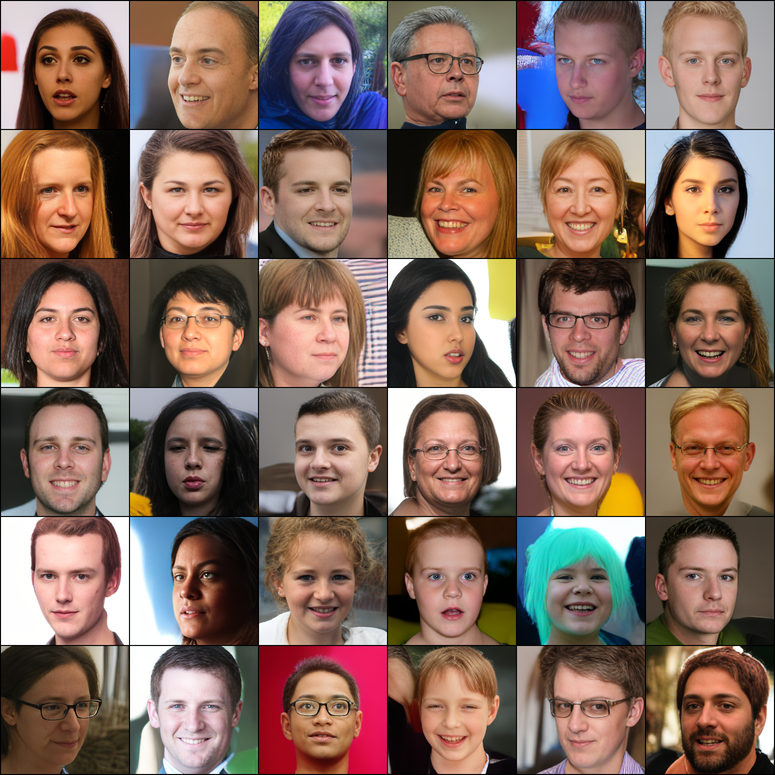
\includegraphics[width=1.0\textwidth]{figures/ffhq256-samples-small.png}
        \caption{
            Non-cherry picked batch of samples from the model trained on FFHQ256.
        }
    \end{subfigure}
    \hfill
    \begin{subfigure}[b]{0.47\textwidth}
        \centering
        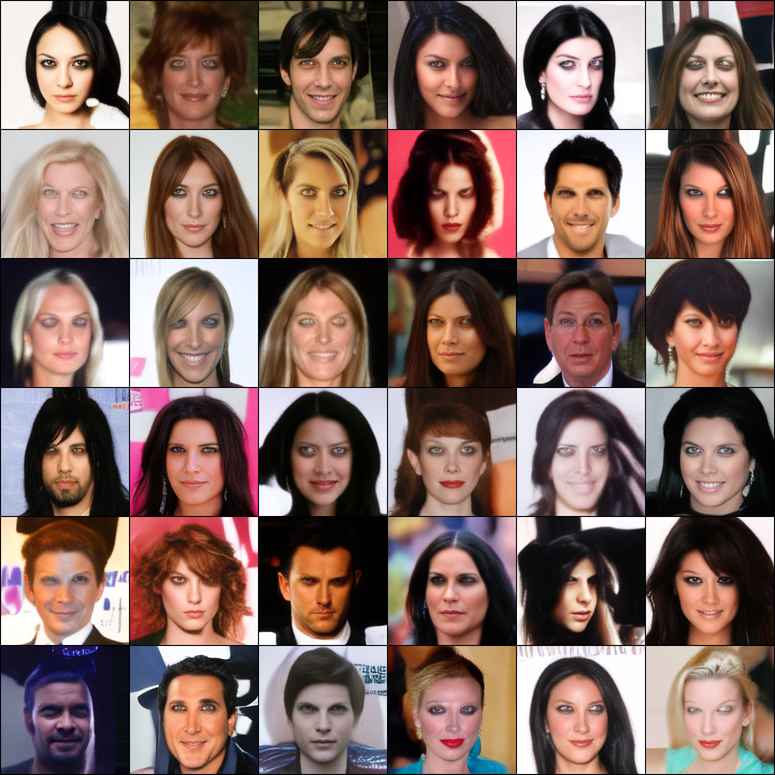
\includegraphics[width=1.0\textwidth]{figures/celeba-samples-small.png}
        \caption{
            Non-cherry picked batch of samples from the model trained on CelebA.
        }
    \end{subfigure}
    \caption{Unconditional generation on $256 \times 256$ face datasets.}
    \label{fig:face}
\end{figure}

\begin{figure}[ht]
    \centering
    \begin{subfigure}[b]{\textwidth}
        \centering
        \includegraphics[width=1.0\textwidth]{figures/nearest-ffhq256.png}
    \end{subfigure}
    \caption{
        FFHQ256 samples and their nearest neighbours in the dataset, based on LPIPS
        perceptual loss. Left-most column is a sample from our trained
        model, followed then by nearest neighbours, increasing in distance
        from left-to-right.
    }
\end{figure}

We evaluate our method on the task of unconditional image generation on datasets
FFHQ256, FFHQ1024, and CelebA. We use pretrained \gls{vqgan} checkpoints
provided by the original \gls{vqgan} authors~\cite{esser2021taming} for $256
\times 256$ experiments. We evaluate our models using FID
Infinity~\cite{chong2020effectively}, coverage, and
density~\cite{ferjad2020icml}, plotting how these metrics change as number of
sampling steps $\markovSteps$ (Figure~\ref{fig:step}), sampling temperature
$\temperature$ (Figure~\ref{fig:temp}), and sample proportion
(Figure~\ref{fig:prop}) are varied. Additionally, we present representative
unconditional samples in Figures~\ref{fig:main} \& \ref{fig:face}.

Figure~\ref{fig:step} demonstrates a surprising property of our model:
additional steps during the sampling process do not improve sample quality
further. It is important to note that this only holds if the other parameters
remain fixed. Therefore, the results do not suggest that additional sampling
steps are always detrimental to performance, as a low number of steps will
clearly result in poor quality results. Rather, it indicates that merely
adding more sampling steps is not sufficient in our framework, and other
parameters must also be adjusted to reflect a higher time budget.

Figure~\ref{fig:temp} shows that picking a temperature in the range of $0.5$ to
$0.7$ leads to best sample quality across a large set of samples, at the cost of
reduced diversity. Our model is capable of sampling with a higher temperature at
the cost of occasionally producing corrupted examples. Figure~\ref{fig:prop}
confirms the result in \citet{savinov2022stepunrolled} that sampling with a
lower proportion leads to higher sample diversity. However, in low-step
scenarios, low proportions cannot be used effectively as the majority of
elements in $\latent_t$ will not have enough opportunities to update, resulting
in low quality outputs.

The result samples shown in Figures~\ref{fig:main} \& \ref{fig:face} demonstrate
that our model is capable of generating high quality and diverse samples. Our
aim was to push the efficiency of generative models to their limit, however we
were still surprised at precisely how fast the model could generate --
particularly on megapixel scale experiments. The samples in
Figure~\ref{fig:main} were created in a two seconds on a GTX 1080Ti. This can be
further improved with more powerful accelerators, further optimisation, and
model compilation. This kind of speed is unparalleled; significantly faster than
prior non-adversarial solutions at this resolution.

\subsection{Conditional Image Generation}
\label{subsec:evaluationConditional}

\begin{figure}[ht]
    \centering
    \begin{subfigure}[b]{0.47\textwidth}
        \centering
        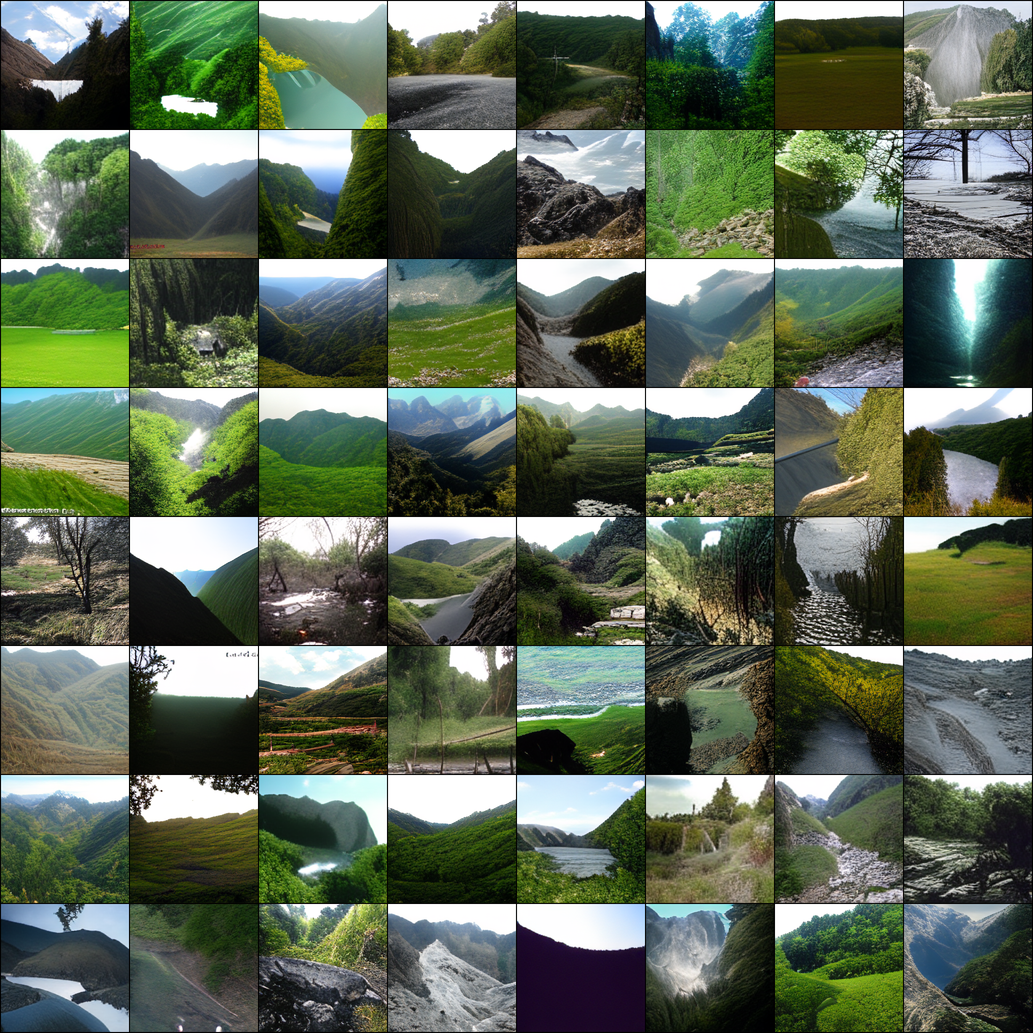
\includegraphics[width=1.0\textwidth]{figures/imagenet-valley-small.png}
        \caption{
            $256 \times 256$ successful samples from the class ``Valley''.}
    \end{subfigure}
    \hfill
    \begin{subfigure}[b]{0.47\textwidth}
        \centering
        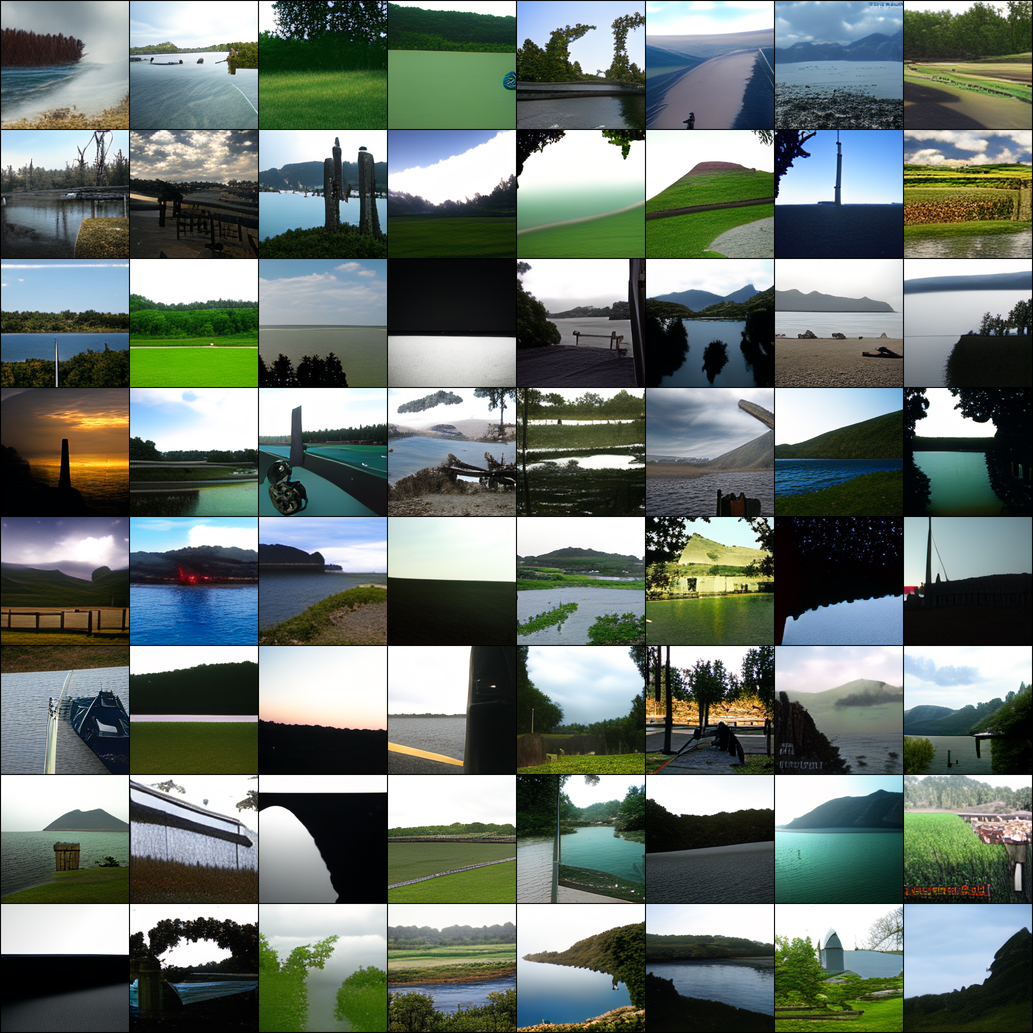
\includegraphics[width=1.0\textwidth]{figures/imagenet-lakeside-small.png}
        \caption{
            $256 \times 256$ successful samples from the class ``Lakeside''.
        }
    \end{subfigure}\\
    \vspace{0.5cm}
    \begin{subfigure}[b]{0.47\textwidth}
        \centering
        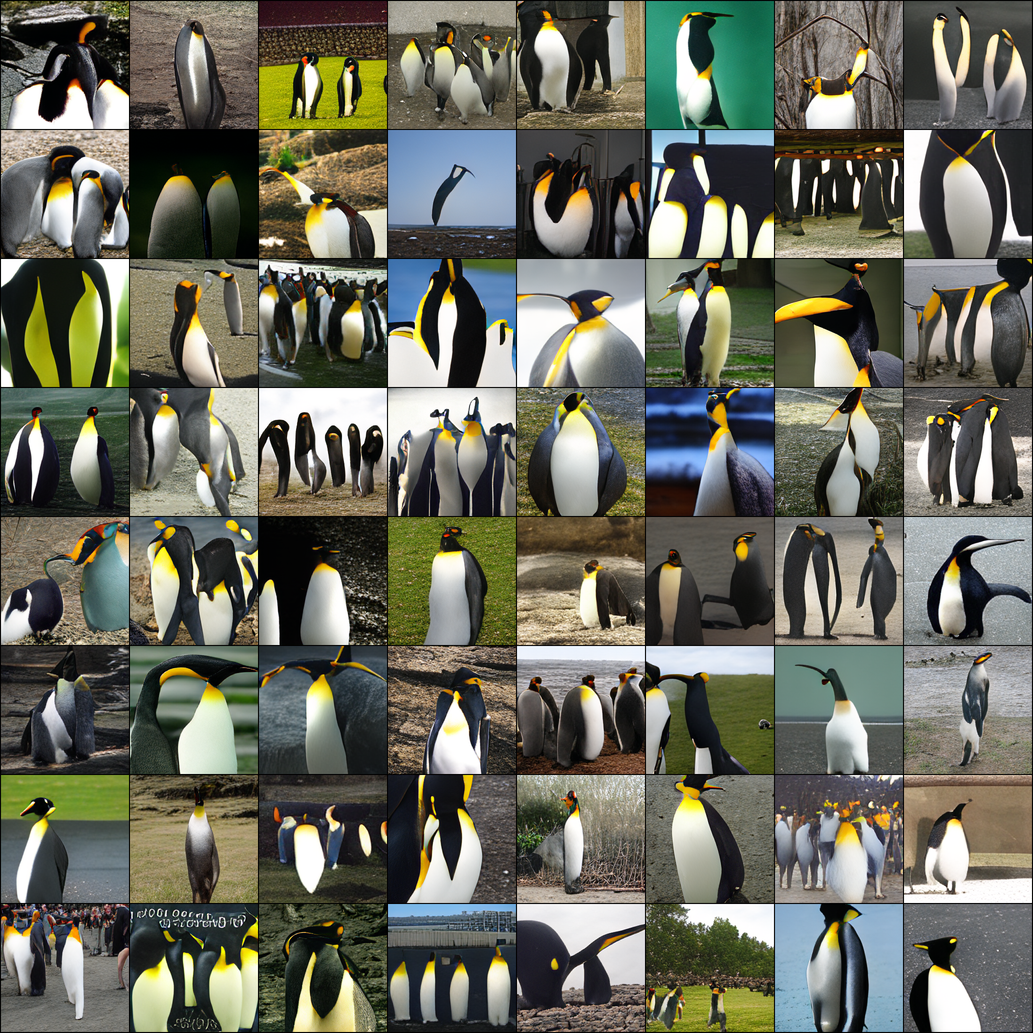
\includegraphics[width=1.0\textwidth]{figures/imagenet-penguin-small.png}
        \caption{
            $256 \times 256$ failed samples from the class ``King Penguin''.
        }
    \end{subfigure}
    \hfill
    \begin{subfigure}[b]{0.47\textwidth}
        \centering
        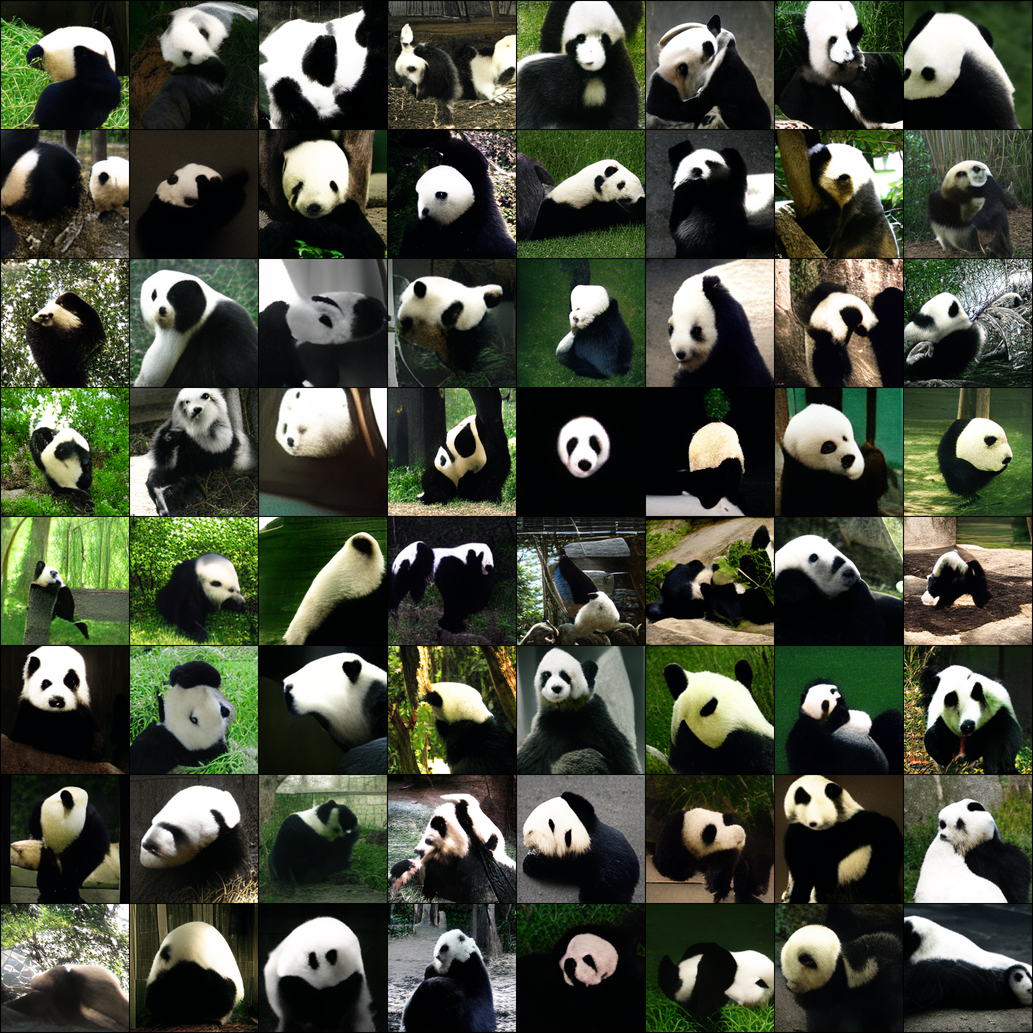
\includegraphics[width=1.0\textwidth]{figures/imagenet-panda-small.png}
        \caption{
            $256 \times 256$ failed samples from the class ``Giant Panda''.
        }
    \end{subfigure}
    \caption{
        Examples of class-conditioned generation on ImageNet256 using
        $\markovSteps = 50$ sampling steps. Top row contains examples of
        successful samples whereas bottom row contains failed samples. The
        contents of the failed samples resemble the target class, but are of low
        quality.
    }
    \label{fig:imagenet}
\end{figure}

\begin{figure}[ht]
    \centering
    \begin{subfigure}[b]{0.47\textwidth}
        \centering
        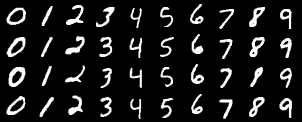
\includegraphics[width=1.0\textwidth]{figures/mnist-samples.png}
        \caption{
            Conditional, pixel-wise generation on MNIST.
        }
    \end{subfigure}
    \hfill
    \begin{subfigure}[b]{0.47\textwidth}
        \centering
        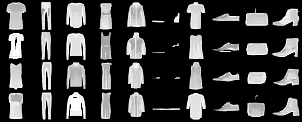
\includegraphics[width=1.0\textwidth]{figures/fashionmnist-samples.png}
        \caption{
            Conditional, pixel-wise generation on Fashion-MNIST.
        }
    \end{subfigure}
    \caption{
        Testing conditional generation using MNIST-style datasets. Coherent
        samples demonstrate that the proposed conditioning method does inject class
        information.
    }
    \label{fig:mnist}
\end{figure}

Another critical component of an ideal generative model is the ability to
control its generation. We explore class-conditioned image generation of
ImageNet at $256 \times 256$ resolution, using the pretrained ImageNet256
\gls{vqgan} checkpoints provided in the original work~\cite{esser2021taming}. 

There are many valid ways of injecting a conditioning signal into generative
models, for example passing one-hot or embedding class vectors. We use a simple
solution proposed in~\cite{parmar2018image} to add a learned class embedding to
every input embedding. To test whether their proposed method can also be applied
to \gls{sundae}, we conducted an experiment on discrete MNIST-style datasets. We
treat each of the possible 8-bit greyscale colour values as a codebook
index, resulting in $\vqganNbLatents = 256$ -- generating pixels directly rather
than image patches. Results of these experiments are shown in
Figure~\ref{fig:mnist} and demonstrate that \gls{sundae} can incorporate using
this simple approach.

Despite this, our model fails to produce reasonable samples for all classes
present in ImageNet. On classes representing large scenes such as landscapes,
the samples are convincing and diverse, however for classes requiring
fine-grained detail the outputs merely resemble the target class. Results of
conditional generation with four representative classes are shown in
Figure~\ref{fig:imagenet}. Due to this, we chose not to compute perceptual
metrics for conditional experiments as the sample quality was clearly
insufficient via inspection alone. This could be a result of lack of model
capacity, lack of training time, or the conditioning strategy tested on MNIST
being insufficient for ImageNet. The training of an effective conditional model
is left for future work.

\subsection{Arbitrary Image Inpainting}
\label{subsec:evaluationInpainting}

\begin{figure}[h]
    \centering
    \begin{subfigure}[b]{\textwidth}
        \centering
        \label{fig:inpaintExample}
        \includegraphics[width=1.0\linewidth]{figures/inpaint.png}
        \caption{A large example of inpainting on a $1024 \times 1024$ image using our
        model.}
    \end{subfigure}
    \\
    \begin{subfigure}[b]{0.47\textwidth}
        \centering
        \includegraphics[width=1.0\textwidth]{figures/inpaint-block/inpaint-variation-small.png}
        \caption{
            Multiple results of inpainting using the same block mask.
        }
    \end{subfigure}
    \hfill
    \begin{subfigure}[b]{0.47\textwidth}
        \centering
        \includegraphics[width=1.0\textwidth]{figures/inpaint-rand/inpaint-variation-small.png}
        \caption{
            Multiple results of inpainting on the same random mask. 
        }
    \end{subfigure}
    \caption{
        Inpainting results on FFHQ1024. We compute multiple outputs per
        input image and mask to demonstrate diversity of outputs. Inpainting
        using a \gls{vq} image model cannot be applied perfectly at a
        pixel-level. Nevertheless, the model still produces many convincing
        outputs at very high resolutions.
    }
\end{figure}

As outlined earlier, \acrlong{nar} generative models have a number of advantages
on inpainting tasks, including supporting arbitrary masks and being able to use
the full context available to them. We provide a number of examples of
inpainting on FFHQ1024, showcasing different patterns and results given the same
starting image and mask. As our method utilises a \gls{vq} image model, it is
incapable of doing fine-grained inpainting at a pixel level. We found in
practise this had little effect on the perceptual quality of the outputs.

\subsection{Limitations}
\label{subsec:evaluationLimitation}

As a result of our evaluation, some limitations of our approach arise. One
crucial weakness is that our \gls{vq} image model still utilises adversarial
components within it. This potentially means that each image patch
(corresponding to each codebook entry) could still suffer from mode collapse
issues. However, our resulting samples are still diverse, suggesting that
patch-wise mode collapse did not have a significant effect on the final samples.

We encountered great instability during training of the large \gls{vqgan} which
led to many failed experiments. Additionally, the extreme compression ratio in
the large \gls{vqgan} model resulted in occasional unrealistic artifacts. Though
most reconstructions are of good quality, the artifacts did rarely appear in the
samples. Further research into high compression \gls{vq} models that do not use
adversarial components remains an open and challenging area of research. When
such a \gls{vq} model is designed, it can easily be substituted into our
proposed framework.

Despite our model demonstrating extremely fast sampling it falls short of many
recent methods in terms of perceptual quality
metrics~\cite{bondtaylor2021unleashing}. Though measures of perceptual quality
such as FID are known to be flawed~\cite{chong2020effectively}, other measures
such as density and coverage also show inferior sample
quality~\cite{ferjad2020icml}. This is especially true on ImageNet where many
classes merely resemble the target class -- though this is likely due to lack of
model capacity and training time. Despite this, the resulting samples on the
FFHQ datasets are still very diverse and of excellent perceptual quality.
Further work, particularly extensive parameter sweeps, is needed to improve
quality in terms of these perceptual metrics.
